\documentclass[a4paper,10pt]{article}

\usepackage{tabularx}
\usepackage{graphicx}
\usepackage{geometry}
\geometry{
    top=2cm,
    bottom=2cm,
    left=1cm,
    right=1cm
}

\usepackage{xepersian}
\settextfont{Vazirmatn-Regular.ttf}

\title{TOMSAC - روش مدیریت تعادل بین ایمنی خودرویی و امنیت سایبری}
\author{}
\date{}

\linespread{1.5}

\begin{document}

    \maketitle

    \begin{abstract}
        
        وابستگی‌های متقابل ایمنی و امنیت برای محققان چندین دهه مورد توجه بوده است. با این حال، در عمل، به دلایل مختلفی از جمله عدم درک کافی و تمایل به تغییر رویه‌های فعلی، توجه لازم به آن‌ها نمی‌شود. این تحقیق با هدف پیشبرد وضعیت هنر در این زمینه با توسعه یک روش عملی، آسان برای انطباق و استفاده برای مدیریت وابستگی‌ها و تعادل‌ها در طول دوره توسعه سیستم‌های سایبر-فیزیکی انجام شده است. این روش به نام TOMSAC که مخفف مدیریت تعادل بین ایمنی و امنیت سایبری است، نامیده شده است.

    \end{abstract}

    \section{مقدمه}

        یک بررسی جامع از روش‌های مهندسی مشترک برای ایمنی و امنیت سایبری در سراسر حوزه سایبر-فیزیکی توسط Kavallieratos و همکاران (2020) ارائه شده است. این مقاله یک بررسی جامع از 68 روش مهندسی مشترک ایمنی و امنیت سایبری ارائه می‌دهد و به مسائل باز و چالش‌های پژوهشی مرتبط می‌پردازد. این 68 روش به دو دسته "یکپارچه" (یعنی دو فرآیند جداگانه مرتبط ایمنی و امنیت) و "ترکیبی" (یعنی یک فرآیند یکپارچه که هم ایمنی و هم امنیت را ترکیب می‌کند) تقسیم می‌شوند. 37 روش از روش‌های بررسی‌شده یکپارچه هستند و 31 روش ترکیبی. بیشتر روش‌های بررسی‌شده مدل‌محور هستند (52 از 68) و برای یک حوزه کاربردی واحد توسعه یافته‌اند (45). تنها 20 روش با استانداردهای مربوطه اطلاعاتی دارند و جالب این است که اکثر روش‌های بررسی‌شده (49) به مسئله حل تضاد نمی‌پردازند. تنها 28 روش شامل تکنیک‌هایی برای ارتباط نتایج با ذینفعان هستند، در حالی که اکثریت (41) توسط هیچ ابزار یا جعبه‌ابزاری پشتیبانی نمی‌شوند. در مجموع، این نتایج نشان می‌دهد که حوزه مهندسی مشترک امنیت سایبری و ایمنی هنوز بالغ نشده است.

        Eames و Moffett (1999) بیان می‌کنند که روش‌هایی که تلاش می‌کنند تحلیل‌های ایمنی و امنیتی را یکپارچه کنند، معایبی دارند و نتیجه‌گیری می‌کنند که "در اکثر موارد تلاش برای یکپارچه‌سازی تحلیل‌های ریسک ایمنی و امنیت نامناسب است." در مورد 'ادغام'، آن‌ها نتیجه می‌گیرند که "ارزش ادغام ایمنی و امنیت در هماهنگ‌سازی تکنیک‌های هر حوزه است." این روش (ادغام) اجازه می‌دهد تا تکنیک‌های تخصصی هر دو حوزه ایمنی و امنیت بدون تغییر باقی بمانند و نیاز به آموزش مجدد تخصص‌های ویژه نباشد.

        پروژه AQUAS Pomante) و همکاران، 2019) با هدف بررسی وابستگی‌های متقابل ایمنی، امنیت و عملکرد در زمینه افزایش پیچیدگی ناشی از اتصال دنیای باز و دنیای تعبیه شده آغاز شد. آن‌ها این کار را در پنج حوزه مختلف (مدیریت ترافیک هوایی، دستگاه‌های پزشکی، واگن‌های ریلی، درایو صنعتی و معماری‌های چند هسته‌ای فضایی) انجام دادند.

        یکی از مشارکت‌های کلیدی AQUAS ارتقا روش‌های ترکیبی برای استانداردها فراتر از وضعیت کنونی بود. این کار با تکامل مفهوم و عملی کردن پرونده‌های ایمنی اطلاع‌رسانی شده توسط امنیت انجام شد که تأثیر آن بر عملکرد در نظر گرفته شده بود. همچنین مفاهیم سیستم‌های سیستم‌ها نیز مورد بررسی قرار گرفت. مقاله AQUAS نزدیک‌ترین به روش ماست که به حوزه خودرویی محدود شده است.

        در زمینه خودرویی، از سال 2013 Bloomfield و همکاران (2013) بر روی "ایمنی اطلاع‌رسانی شده توسط امنیت" بر اساس تأثیر امنیت بر پرونده‌های ایمنی ساختاری کار می‌کردند. آن‌ها به چالش‌های موجود در هم‌کاری ایمنی و امنیت، از جمله نیاز به یک هستی‌شناسی مشترک، تفاوت‌های اصول زیربنایی این حوزه‌ها، مدل‌های تهدید متفاوت و نیاز به یک رویکرد مشترک به استانداردهای ایمنی و امنیت اشاره می‌کنند. این علاقه منجر به نگارش کد رفتار BSI PAS:11281 توسط Robin Bloomfield و دیگران از شرکت او شد تا "توصیه‌هایی برای مدیریت ریسک‌های امنیتی که ممکن است به مصالحه ایمنی در اکوسیستم خودروی متصل منجر شوند" ارائه دهد (مؤسسه استاندارد بریتانیا، 2018).

        اخیراً، امنیت سایبری برای چندین دسته وسیله نقلیه از جمله خودروهای سواری، اتوبوس‌ها و کامیون‌ها به یک حوزه تحت نظارت تبدیل شده است. مقررات UN 155 ،UNECE) (2021a 156 و ،UNECE) (2021b به ترتیب الزامات امنیت سایبری و به‌روزرسانی نرم‌افزار را مشخص می‌کنند که تولیدکنندگان باید برای دریافت تایید نوع برای آن وسایل نقلیه در کشورهایی که مقررات را اجرا می‌کنند، رعایت کنند. به ویژه، اتحادیه اروپا UN R155 را به عنوان بخشی از مقررات ایمنی عمومی (GSR2) اجرا کرده است که نقش مهم امنیت سایبری در ایمنی کلی را بیشتر تأیید می‌کند. رعایت R155 همچنین به عنوان بخشی از دیگر مقررات UNECE از جمله R157 ،UNECE) (2021c در مورد تایید نوع سیستم‌های حفظ خط خودکار (ALKS) لازم است که نیاز به در نظر گرفتن "حملات سایبری که بر ایمنی خودرو تأثیر می‌گذارند" را دارد.

        در آگوست 2021، استاندارد بین‌المللی جدید \lr{ISO/SAE 21434} "خودروهای جاده‌ای - مهندسی امنیت سایبری" ،ISO/SAE) (2021a منتشر شد تا از اجرای عملی UN R155 پشتیبانی کند. این سند توسط کارشناسان صنعت خودرویی شامل تولیدکنندگان خودرو، زنجیره تامین طبقه‌بندی‌شده، مشاوران امنیت سایبری و سازمان‌های دولتی توسعه یافت. اکنون در صنعت خودرویی به عنوان وضعیت هنر برای مهندسی امنیت سایبری به طور گسترده‌ای استفاده می‌شود، که راهنمایی در مورد اجرای یک سیستم مدیریت امنیت سایبری و انجام فعالیت‌های امنیت سایبری مورد نیاز برای رعایت UN R155 ارائه می‌دهد. \lr{ISO/SAE 21434} به صراحت از سازمان‌ها می‌خواهد که دیگر رشته‌های مهندسی که با امنیت سایبری در تعامل هستند، مانند ایمنی عملکردی، را شناسایی کنند و کانال‌های ارتباطی بین آن رشته‌ها را ایجاد کنند. علاوه بر این، استاندارد بین‌المللی \lr{ISO 26262} برای ایمنی عملکردی ،ISO) 2018) شامل یک الزام متقابل برای شناسایی تعاملات و ایجاد کانال‌های ارتباطی بین ایمنی عملکردی و امنیت سایبری است. رابطه قوی به ویژه بین امنیت سایبری و ایمنی عملکردی در نحوه اشتراک‌گذاری عناصر مشترک از چارچوب‌های فرآیندی که این دو استاندارد تعریف می‌کنند، دیده می‌شود، برای مثال مراحل چرخه حیات هماهنگ و رویکرد مدیریت ریسک.

        در حوزه خودرویی، اولین منطقه‌ای که تعادل ایمنی / امنیت سایبری مشهود شد، حوزه bus CAN بود. این باس برای ارتباط بین واحدهای کنترل الکترونیکی (ECU) طراحی شده بود. این باس بدون در نظر گرفتن امنیت و با قابلیت اطمینان بسیار بالا تعریف شد. Kleberger و همکاران (2011) یک مرور کلی از تهدیدات امنیتی درون خودرو و حفاظت‌های بالقوه با توجه به شبکه CAN ارائه می‌دهند.

        اصالت یک نیاز امنیتی مهم برای سیستم‌های خودرویی است و بسیاری از راه‌حل‌های نرم‌افزاری یا سخت‌افزاری احراز هویت در Kleberger و همکاران (2011) بررسی شده‌اند. از این راه‌حل‌ها، کد احراز هویت پیام (MAC) تکنیک اصلی است. پهنای باند محدود و اندازه بار مفید پروتکل CAN به این معناست که این تکنیک‌ها باید سبک‌وزن باشند تا نیازهای دیگر طراحی را برآورده کنند. از آنجایی که CAN در درجه اول یک پروتکل طراحی شده برای ایمنی است، این را می‌توان به عنوان یک گام اولیه در تعادل بین نیازهای ایمنی و امنیت در نظر گرفت.
        
        Lin و Yu (2016) مرور خوبی از تعادل‌های ایمنی و امنیت با بررسی TTEthernet (اترنت زمان‌مند) ارائه می‌دهند. این به عنوان یکی از رقبای جایگزین برای bus CAN دیده می‌شود، اگرچه نویسندگان از TTEthernet به عنوان یک رسانه ارتباطی بین خودروها، نه داخل آن‌ها، استفاده می‌کنند. آن‌ها به سه کاربرد نگاه می‌کنند: مدیریت کلید مخفی، تکرار و حذف فریم، و تقسیم‌بندی شبکه محلی مجازی .(VLAN)
        
        Apvrille و Li (2019) بر این اساس کار می‌کنند که یک فرد (یا یک تیم) مسئول طراحی اولیه سیستم است و بنابراین هماهنگ کردن نیازهای ایمنی، امنیت و عملکرد نسبتاً ساده است. TTool ،Apvrille) 2008) (ابزار انتخابی آن‌ها) کل فرآیند مدل‌سازی و تایید را در یک جعبه ابزار واحد نگه می‌دارد که به طور همزمان برای نیازهای ایمنی، امنیت و عملکرد انجام می‌شود. Apvrille و Li (2019) اشاره می‌کنند که صحت تبدیل مدل برای ProVerif تا حدی ثابت شده است. آن‌ها همچنین اکتشاف فضای طراحی را در کار خود ارائه می‌دهند. اما با نگاه جداگانه به امنیت، ایمنی و عملکرد، به نظر می‌رسد که آن‌ها فرصت بهره‌برداری از وابستگی‌های متقابل بین این موارد را از دست می‌دهند. آن‌ها پیشنهاد می‌دهند که یکی از امنیت، ایمنی یا عملکرد به عنوان نیاز اصلی ابزار در نظر گرفته شود و راه‌هایی برای رسیدگی به عناصر غیرمطلوب از دو مورد دیگر ارائه کنند. این نشان می‌دهد که مقاله (اگرچه در مطالعه موردی از خودروها استفاده می‌کند) در حال حاضر در واقع بر بخش‌های کوچکتر CPS متمرکز است. کار ما در حال حاضر به شدت بر خودروها متمرکز است و ما به پرسش مقایسه روابط متقابل ایمنی و امنیت از دیدگاه آن‌ها می‌پردازیم.

        با نگاهی گسترده‌تر به فناوری‌های ارتباطی، در Huber و همکاران (2018) نویسندگان بررسی می‌کنند که چگونه سازمان‌های صنعت خودروسازی با چالش ادغام جنبه‌های ایمنی و امنیت در طول توسعه سیستم مقابله می‌کنند. نتیجه‌گیری کلی آن‌ها این است که در حال حاضر "کمبودهای قابل توجهی در ادغام هر دو حوزه وجود دارد." نویسندگان یک بررسی اکتشافی (محدود به اروپا) از ادغام جنبه‌های ایمنی و امنیت در طول توسعه سیستم در صنعت خودروسازی ارائه می‌دهند. چهار یافته کلیدی (KF) از این مطالعه به دست آمده است:

        \begin{itemize}
            
            \item اکثریت سازمان‌های (خودروسازی) به طور فعال وابستگی‌های متقابل بین نیازهای ایمنی و امنیت را در نظر نمی‌گیرند.

            \item مشکلات رایج مربوط به پیچیدگی، مدیریت تغییر ردیابی و در دسترس بودن منابع، ادغام امنیت را پیچیده می‌کنند.

            \item اهداف هر دو حوزه امنیت و ایمنی در چندین سازمان گسترده می‌شوند.

            \item درک نسبتاً یکنواخت و آگاهی عمومی در سازمان‌ها در مورد تفاوت‌های اساسی بین حوزه‌های ایمنی و امنیت وجود دارد.

        \end{itemize}

        نتیجه‌گیری از این یافته‌های کلیدی نیاز به یک مدل جامع است که اسناد و مدارک را یکپارچه کند تا پیچیدگی را کاهش داده و مدیریت تغییرات موثر را تسهیل کند.

        چهار نوع تعامل بین ایمنی و امنیت توسط Piètre-Cambacédès (2010) (به زبان فرانسوی) معرفی شده و سپس توسط Kriaa و همکاران (2015) منتشر شده است. این تعاملات شامل موارد زیر هستند:

        \begin{itemize}
            
            \item وابستگی شرطی: برآورده شدن نیازهای ایمنی یک شرط برای امنیت است یا برعکس.

            \item تقویت متقابل: نیازها یا اقدامات ایمنی امنیت را افزایش می‌دهند یا برعکس.

            \item تقابل: نیازها یا اقدامات ایمنی و امنیتی با یکدیگر در تضاد هستند.

            \item استقلال: هیچ تعاملی وجود ندارد.

        \end{itemize}

        Kolb و همکاران (2021) استدلال می‌کنند که تعاریف دقیق‌تری از ایمنی و امنیت سایبری لازم است، که شامل موارد زیر باشد:

        \begin{itemize}
            
            \item جهت‌گیری: آیا ایمنی و امنیت یک‌طرفه هستند یا دوطرفه و از کدام جهت جریان دارند؟

            \item شدت: برای یک هم‌تحلیل کمی، شدت این تعاملات باید در نظر گرفته شود.

            \item ماهیت تعامل: برای هر یک از تعاملات ممکن، از تأثیر تا وابستگی یا تقابل، در نظر گرفتن تأثیر مثبت یا منفی چنین تعاملی اساسی است. علاوه بر این، وابستگی‌های شرطی سوالی را در مورد اینکه چه کسی مسئول اقدامات است هنگامی که ایمنی و امنیت به شدت وابسته هستند، مطرح می‌کند.

        \end{itemize}

        Kolb و همکاران (2021) تحلیل مقایسه‌ای از 14 روش برای هم‌تحلیل مدل‌محور ایمنی و امنیت انجام دادند. یافته‌ها/چالش‌های کلیدی شامل موارد زیر است:

        \begin{itemize}
            
            \item بیشتر روش‌ها درخت‌های حمله و درخت‌های خطا را ترکیب می‌کنند.

            \item هیچ ساختار جدیدی برای ثبت تعاملات ایمنی-امنیت معرفی نشده است. در عوض، ساختارهای موجود برای مدل‌سازی ایمنی و امنیت با هم ترکیب شده‌اند.

            \item تعاملات ایمنی و امنیت هنوز به طور کامل درک نشده‌اند.

            \item هیچ معیار جدیدی برای کمّی کردن تعاملات ایمنی-امنیت پیشنهاد نشده است.

            \item هیچ مطالعه موردی بزرگ در مورد هم‌تحلیل ایمنی/امنیت انجام نشده است.

        \end{itemize}

        هدف کلی تحقیقات ما ادامه رسیدگی به این چالش‌ها است.

    \section{امنیت و وابستگی متقابل امنیت سایبری}

        شکل 1 و شکل 2 وابستگی‌های متقابل بین اقدامات و نیازهای ایمنی و امنیت سایبری را نشان می‌دهند. شکل 1 تأثیر اقدامات ایمنی بر امنیت سایبری را نشان می‌دهد، در حالی که شکل 2 تأثیر اقدامات امنیت سایبری بر ایمنی را نمایش می‌دهد. سه نوع رابطه که در Piètre-Cambacédès (2010) و Kriaa و همکاران (2015) تعریف شده‌اند، در شکل 1 و شکل 2 به تصویر کشیده شده‌اند: تقابل، تقویت، و وابستگی شرطی.

        \begin{table}
            
            \centering
            \begin{tabular}{ c c }
            
                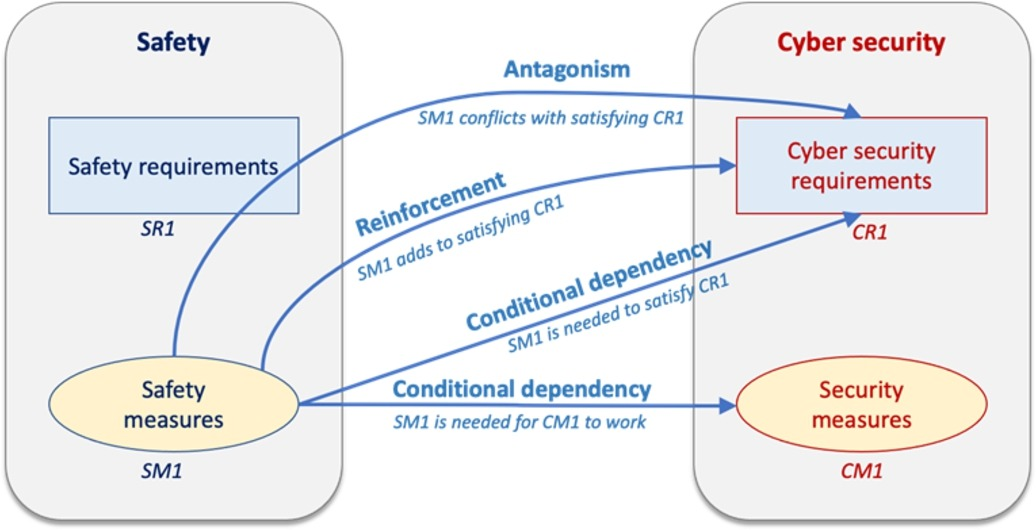
\includegraphics[width=0.5\textwidth]{Image/fig1.jpg}

                &

                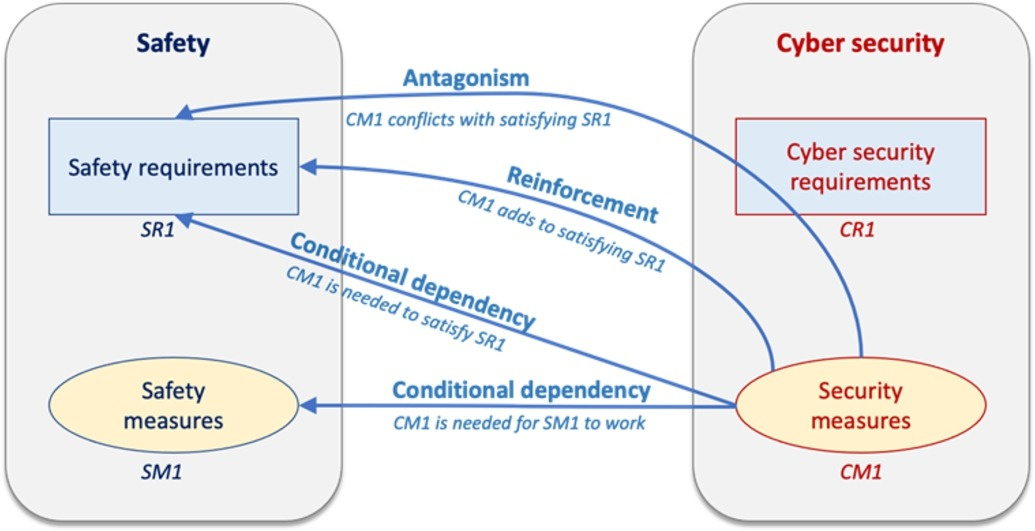
\includegraphics[width=0.5\textwidth]{Image/fig2.jpg} \\

                شکل 1: تاثیر اقدامات ایمنی بر امنیت سایبری

                &

                شکل 2: تاثیر اقدامات امنیت سایبری بر ایمنی
                        
            \end{tabular}

        \end{table}

        علاوه بر وابستگی‌های متقابل بین نیازها و اقدامات ایمنی و امنیت سایبری، ممکن است وابستگی‌هایی بین سطوح خرابی و حمله نیز وجود داشته باشد. به عنوان مثال، یک خرابی ایمنی می‌تواند به فعال‌سازی یک حمله امنیتی کمک کند، یا برعکس. علاوه بر این، یک خرابی ایمنی می‌تواند یک حمله امنیتی را مسدود کند، یا برعکس. بنابراین، دو نوع رابطه جدید می‌توان تعریف کرد: "فعال‌سازی" و "مسدودسازی". ما طبقه‌بندی اولیه وابستگی‌های متقابل ایمنی و امنیت، که توسط Kolb و همکاران (2021) پیشنهاد شده بود، را گسترش داده و روابط "فعال‌سازی" و "مسدودسازی" را اضافه کرده‌ایم، همان‌طور که در شکل 3 نشان داده شده است.

        \begin{table}
            
            \centering
            \begin{tabular}{ c }
                
                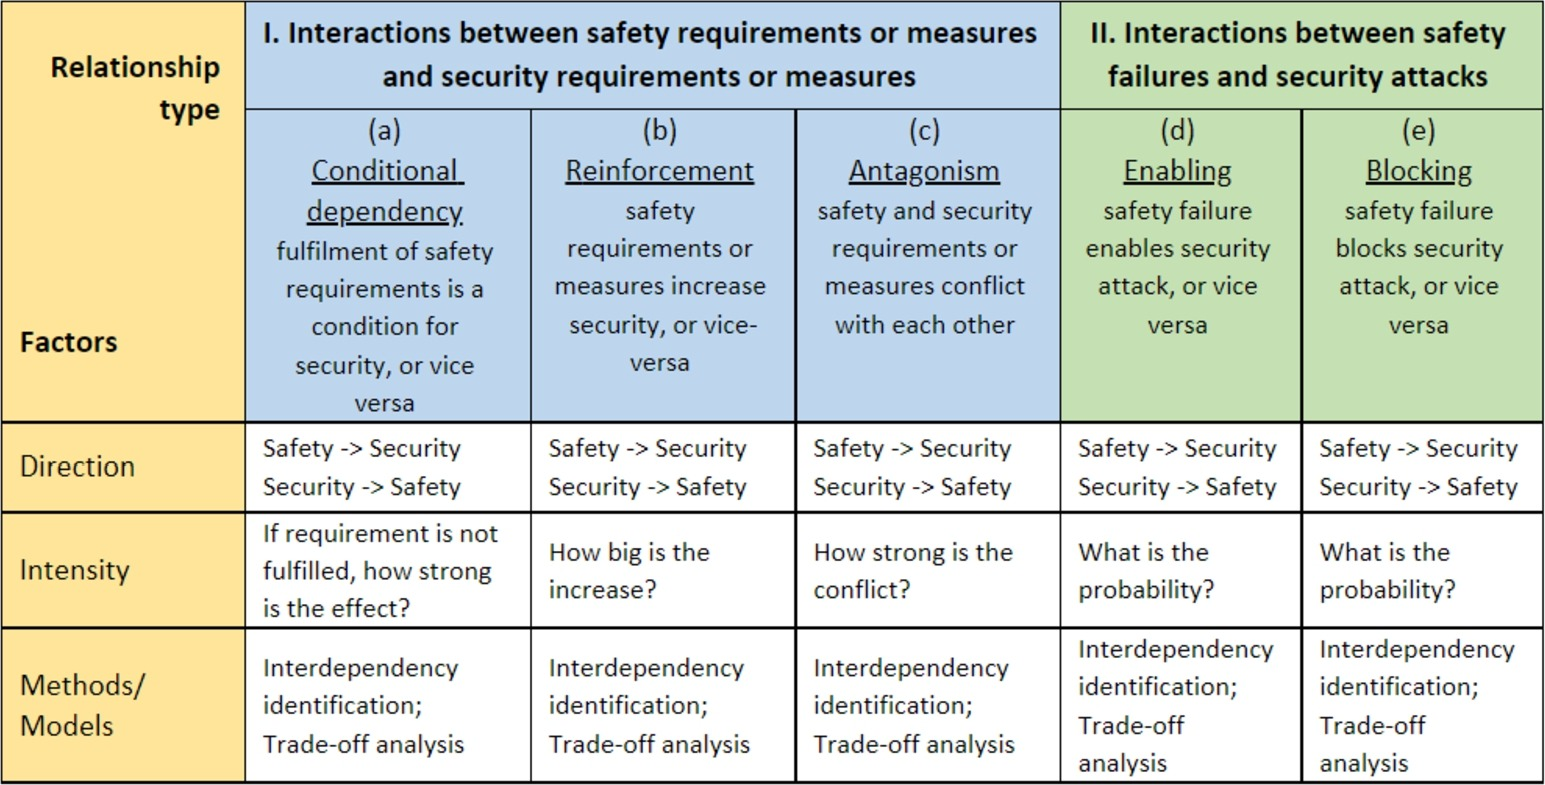
\includegraphics[width=1\textwidth]{Image/fig3.jpg} \\

                شکل 3: امنیت و وابستگی متقابل امنیتی

            \end{tabular}

        \end{table}

        علاوه بر انواع روابط، شکل 3 شامل عوامل مختلفی است که برای تمامی انواع روابط مرتبط هستند، مانند:
        
        \begin{itemize}
            
            \item جهت – دو جهت وجود دارد، یا از ایمنی به امنیت (تأثیر ایمنی بر امنیت) یا برعکس
            
            \item شدت – اندازه‌گیری شدت وابستگی متقابل.

            \item روش‌ها/مدل‌ها – روش‌ها و مدل‌های مختلف برای تسهیل تحلیل وابستگی‌های متقابل

        \end{itemize}

        هدف کار ما ارائه روشی است که به بررسی رابطه بین ایمنی و امنیت سایبری در هر مرحله از چرخه حیات سیستم سایبر فیزیکی (CPS) بپردازد و تعامل بین آن‌ها را برجسته کند.

    \section{مروری بر روش‌شناسی}

        شکل 5 چارچوب روش‌شناسی TOMSAC را نشان می‌دهد که شامل موارد زیر است:
    
        \begin{itemize}
            
            \item مراحل چرخه حیات CPS

            \item تیم‌های درگیر در فرآیند توسعه، مانند تیم‌های طراحی/توسعه، ایمنی و امنیت   سایبری، تأمین‌کنندگان و کاربران؛

            \item نقاط هماهنگی در مراحل مختلف چرخه حیات برای تیم‌ها به منظور هماهنگ کردن محصولات کاری خود و انجام مبادلات، در صورت لزوم.

        \end{itemize}

        تیم‌های متعددی در توسعه CPS درگیر هستند، مانند توسعه‌دهندگان، تیم ایمنی، تیم امنیت سایبری و غیره، که هر کدام استانداردهای خود را دنبال می‌کنند، فرآیندهای مختلفی دارند، محصولات کاری مختلفی توسعه می‌دهند و حتی به زبان‌های مختلفی صحبت می‌کنند یا از اصطلاحات مشابه برای معانی مختلف استفاده می‌کنند، که این امر باعث می‌شود درک کامل یکدیگر و یکپارچه‌سازی نتایج کارشان دشوار باشد. هدف روش‌شناسی TOMSAC فراهم کردن یک چارچوب یکپارچه برای این تیم‌ها است تا ارتباط و هماهنگی کارهایشان را تسهیل کند.
        
\end{document}